%package list
\documentclass{article}
\usepackage[top=3cm, bottom=3cm, outer=3cm, inner=3cm]{geometry}
\usepackage{multicol}
\usepackage{graphicx}
\usepackage{url}
%\usepackage{cite}
\usepackage{hyperref}
\usepackage{array}
%\usepackage{multicol}
\newcolumntype{x}[1]{>{\centering\arraybackslash\hspace{0pt}}p{#1}}
\usepackage{natbib}
\usepackage{pdfpages}
\usepackage{multirow}
\usepackage[normalem]{ulem}
\useunder{\uline}{\ul}{}
\usepackage{svg}
\usepackage{xcolor}
\usepackage{listings}
\lstdefinestyle{ascii-tree}{
	literate={├}{|}1 {─}{--}1 {└}{+}1 
}
\lstset{basicstyle=\ttfamily,
	showstringspaces=false,
	commentstyle=\color{red},
	keywordstyle=\color{blue}
}
%\usepackage{booktabs}
\usepackage{caption}
\usepackage{subcaption}
\usepackage{float}
\usepackage{array}

\newcolumntype{M}[1]{>{\centering\arraybackslash}m{#1}}
\newcolumntype{N}{@{}m{0pt}@{}}


%%%%%%%%%%%%%%%%%%%%%%%%%%%%%%%%%%%%%%%%%%%%%%%%%%%%%%%%%%%%%%%%%%%%%%%%%%%%
%%%%%%%%%%%%%%%%%%%%%%%%%%%%%%%%%%%%%%%%%%%%%%%%%%%%%%%%%%%%%%%%%%%%%%%%%%%%
\newcommand{\itemEmail}{jchuraaca@unsa.edu.pe}
\newcommand{\itemStudent}{Julio Rubén Chura Acabana}
\newcommand{\itemCourse}{ F. de Programción 2}
\newcommand{\itemCourseCode}{20230472}
\newcommand{\itemSemester}{I}
\newcommand{\itemUniversity}{Universidad Nacional de San Agustín de Arequipa}
\newcommand{\itemFaculty}{Facultad de Ingeniería de Producción y Servicios}
\newcommand{\itemDepartment}{Departamento Académico de Ingeniería de Sistemas e Informática}
\newcommand{\itemSchool}{Escuela Profesional de Ingeniería de Sistemas}
\newcommand{\itemAcademic}{2023 - B}
\newcommand{\itemInput}{Del 18 Septiembre 2023}
\newcommand{\itemOutput}{Al 20 Septiembre 2023}
\newcommand{\itemPracticeNumber}{02}
\newcommand{\itemTheme}{Arreglos Estandar}
%%%%%%%%%%%%%%%%%%%%%%%%%%%%%%%%%%%%%%%%%%%%%%%%%%%%%%%%%%%%%%%%%%%%%%%%%%%%
%%%%%%%%%%%%%%%%%%%%%%%%%%%%%%%%%%%%%%%%%%%%%%%%%%%%%%%%%%%%%%%%%%%%%%%%%%%%

\usepackage[english,spanish]{babel}
\usepackage[utf8]{inputenc}
\AtBeginDocument{\selectlanguage{spanish}}
\renewcommand{\figurename}{Figura}
\renewcommand{\refname}{Referencias}
\renewcommand{\tablename}{Tabla} %esto no funciona cuando se usa babel
\AtBeginDocument{%
	\renewcommand\tablename{Tabla}
}

\usepackage{fancyhdr}
\pagestyle{fancy}
\fancyhf{}
\setlength{\headheight}{30pt}
\renewcommand{\headrulewidth}{1pt}
\renewcommand{\footrulewidth}{1pt}
\fancyhead[L]{\raisebox{-0.2\height}{
\includegraphics[width=3cm]{img/logo_episunsa.png}}}
\fancyhead[C]{\fontsize{7}{7}\selectfont	\itemUniversity \\ \itemFaculty \\ \itemDepartment \\ \itemSchool \\ \textbf{\itemCourse}}
\fancyhead[R]{\raisebox{-0.2\height}{
\includegraphics[width=1.2cm]{img/logo_abet}}}
\fancyfoot[L]{Estudiante Julio Rubén Chura Acabana}
\fancyfoot[C]{\itemCourse}
\fancyfoot[R]{Página \thepage}

% para el codigo fuente
\usepackage{listings}
\usepackage{color, colortbl}
\definecolor{dkgreen}{rgb}{0,0.6,0}
\definecolor{gray}{rgb}{0.5,0.5,0.5}
\definecolor{mauve}{rgb}{0.58,0,0.82}
\definecolor{codebackground}{rgb}{0.95, 0.95, 0.92}
\definecolor{tablebackground}{rgb}{0.8, 0, 0}

\lstset{frame=tb,
	language=bash,
	aboveskip=3mm,
	belowskip=3mm,
	showstringspaces=false,
	columns=flexible,
	basicstyle={\small\ttfamily},
	numbers=none,
	numberstyle=\tiny\color{gray},
	keywordstyle=\color{blue},
	commentstyle=\color{dkgreen},
	stringstyle=\color{mauve},
	breaklines=true,
	breakatwhitespace=true,
	tabsize=3,
	backgroundcolor= \color{codebackground},
}

\begin{document}
	
	\vspace*{10px}
	
	\begin{center}	
		\fontsize{17}{17} \textbf{ Informe de Laboratorio \itemPracticeNumber}
	\end{center}
	\centerline{\textbf{\Large Tema: \itemTheme}}
	%\vspace*{0.5cm}	
	
	\begin{flushright}
		\begin{tabular}{|M{2.5cm}|N|}
			\hline 
			\rowcolor{tablebackground}
			\color{white} \textbf{Nota}  \\
			\hline 
			\\[30pt]
			\hline 			
		\end{tabular}
	\end{flushright}	
	
	\begin{table}[H]
		\begin{tabular}{|x{4.7cm}|x{4.8cm}|x{4.8cm}|}
			\hline 
			\rowcolor{tablebackground}
			\color{white} \textbf{Estudiante} & \color{white}\textbf{Escuela}  & \color{white}\textbf{Asignatura}   \\
			\hline 
			{\itemStudent \par \itemEmail} & \itemSchool & {\itemCourse \par Semestre: \itemSemester \par Código: \itemCourseCode}     \\
			\hline 			
		\end{tabular}
	\end{table}		
	
	\begin{table}[H]
		\begin{tabular}{|x{4.7cm}|x{4.8cm}|x{4.8cm}|}
			\hline 
			\rowcolor{tablebackground}
			\color{white}\textbf{Laboratorio} & \color{white}\textbf{Tema}  & \color{white}\textbf{Duración}   \\
			\hline 
			\itemPracticeNumber & \itemTheme & 04 horas   \\
			\hline 
		\end{tabular}
	\end{table}
	
	\begin{table}[H]
		\begin{tabular}{|x{4.7cm}|x{4.8cm}|x{4.8cm}|}
			\hline 
			\rowcolor{tablebackground}
			\color{white}\textbf{Semestre académico} & \color{white}\textbf{Fecha de inicio}  & \color{white}\textbf{Fecha de entrega}   \\
			\hline 
			\itemAcademic & \itemInput &  \itemOutput  \\
			\hline 
		\end{tabular}
	\end{table}
	
	\section{Tarea}
	\begin{itemize}		
		\item 
		En este ejercicio se le solicita a usted implementar el juego del ahorcado utilizando el código parcial que 
		se le entrega.
		\item Usted debe realizar varios commits y al término de la actividad deberá realizar un informe
		
	\end{itemize}
	
	\section{Equipos, materiales y temas utilizados}
	\begin{itemize}
		\item Sistema Operativo Windows
		\item VIM 9.0.
		\item OpenJDK 64-Bits 17.0.7.
		\item Git 2.39.2.
		\item Cuenta en GitHub con el correo institucional.
		\item Arreglos Estándar
	\end{itemize}
	
	\section{URL de Repositorio Github}
	\begin{itemize}
		\item URL del Repositorio GitHub para clonar o recuperar.
		\item \url{https://github.com/JulioChura/fp2-23b.git}
		\item URL para el laboratorio 01 en el Repositorio GitHub.
		\item \url{https://github.com/JulioChura/fp2-23b/tree/main/fase01/lab02}
	\end{itemize}
	
	\section{Actividades con el repositorio GitHub}
	
	\subsection{Commits}
	
	\begin{lstlisting}[language=bash,caption={Primer Commit Creando archivo Ejercicio02.java con el código incompleto }][H]
		cd fase01/lab02
		vim Ejercicio02.java
		git add Ejercicio02.java
		git commit -m "Codigo incompleto del juego de El ahorcado"			
		git push -u origin main
	\end{lstlisting}
	
	\begin{lstlisting}[language=bash,caption={Completando el método ingreseLetra }][H]
		vim Ejercicio02.java
	\end{lstlisting}
	\begin{itemize}	
		\item En el código base, la mayor parte del método está completo, sin embargo falta validar si el carácter ingresado es una letra, por lo que en la parte del while, se agrega como condición que mientras la variable laLetra no sea una letra, se seguirá insistiendo al usuario que ingrese dicho valor de manera correcta. 
		\item Para lograr dicha validación, se recurre a los método Character.isLetter(char c) y charAt(int i).
	\end{itemize}	
	\begin{figure}[H]
		\centering
		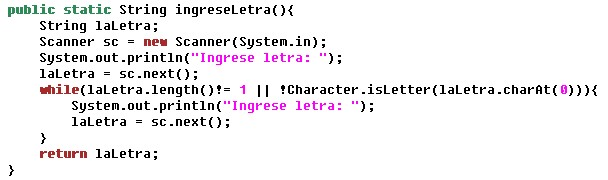
\includegraphics[width=0.8\textwidth,keepaspectratio]{img/metodoIngreseLetra.jpg}
		%\includesvg{img/automata.svg}
		%\label{img:mot2}
		%\caption{Product backlog.}
	\end{figure}
	
	\begin{lstlisting}[language=bash,caption={Probando el método ingreseLetra}][H]
		javac Ejercicio02.java
		java Ejercicio02.java
		+---+
		|   |
		|
		|
		|
		|
		=========
		_ _ _ _ _ _ _ _ _ _ _ _
		
		Ingrese letra:
		2
		Ingrese letra:
		l
	
	\end{lstlisting}
	\begin{lstlisting}[language=bash,caption={Commit: Subiendo al repositorio Ejercicio02.java}][H]
		git add .
		git commit -m "Metodo ingreseLetra() completo"			
		git push -u origin main
	\end{lstlisting}
	
	\begin{lstlisting}[language=bash,caption={Completando el método letraEnPalabraSecreta }][H]
		vim Ejercicio02.java
	\end{lstlisting}
	\begin{itemize}	
		\item En el código base, este método está vacío, por lo que se debe completar. 
		\item Este método básicamente recibe dos parámetros, un String que es el valor que el usuario ingresa y el otro sería la palabra que se extrajo del arreglo de palabras iniciales, para implementar el código, se recurre a un ciclo for el cual recorre la palabra elegida extrayendo los carácteres de dicha palabra y comparándo cada una con el caracter ingresado por el usuario. Para comparar la letra (dato de tipo String) y el carácter extraído de la palabra (dato de tipo char) se opta por convertir el carácter en String usando el método Character.toStrng(char c) para luego usar equasl() el cual compara String. Si hay coincidencias se retorna true, de lo contrario se retorna false
	\end{itemize}
	\begin{figure}[H]
		\centering
		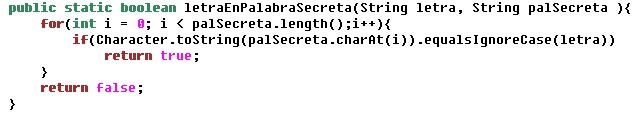
\includegraphics[width=0.8\textwidth,keepaspectratio]{img/letraEnPalabraSecreta.jpg}
		%\includesvg{img/automata.svg}
		%\label{img:mot2}
		%\caption{Product backlog.}
	\end{figure}
	
	
	
	\begin{lstlisting}[language=bash,caption={Commit: Subiendo al repositorio Ejercicio02.java}][H]
		git add .
		git commit -m "Metodo letraEnPalabraSecreta realizado"			
		git push -u origin main
	\end{lstlisting}	
	
	
	
	\begin{lstlisting}[language=bash,caption={Creando un nuevo método que genera un arreglo de Strings formado por Subguiones}][H]
		vim Ejercicio02.java
	\end{lstlisting}
	
	\begin{itemize}	
		\item En el código base, este método no está implementado. 
		\item Este método se encarga de generar un arreglo de Subguiones, el tamaño es de acuerdo a la palabra elegida, el propósito de este método es que el arreglo que se forme formará parte del parámetro del método mostrarBlancosActualizados
	\end{itemize}
	
	\begin{figure}[H]
		\centering
		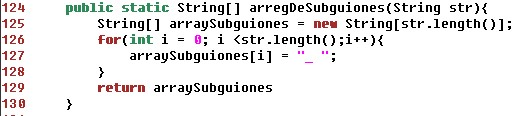
\includegraphics[width=0.8\textwidth,keepaspectratio]{img/arregloSubguiones.jpg}
		%\includesvg{img/automata.svg}
		%\label{img:mot2}
		%\caption{Product backlog.}
	\end{figure}
	
	\begin{lstlisting}[language=bash,caption={Commit: Creando un método que genera un arreglo de subguiones de con tamaño de acuerdo a la palabra elegida }][H]
		git add Ejercicio02.java
		git commit -m "Creando un metodo que genera un arreglo de subguiones de con tamano de acuerdo a la palabra elegida"
	\end{lstlisting}

	
	\begin{lstlisting}[language=bash,caption={Corrigiendo los parámatros del método mostrarBlancosActualizados}][H]
		vim Ejercicio02.java
	\end{lstlisting}
	
	\begin{itemize}	
		\item En el código base, este método recibe como único parámetro un String el cual es la letra que el usuario ingresa. 
		\item El método así como está, no aporta mucho a la solución del problema, es por ello que decido agregarle dos parámetros más, los cuales son un arreglo de String (este arreglo es el de los Subguiones) y adicionalmente se le agrega un String (se trata de la palabra elegida)
	\end{itemize}
	
	\begin{figure}[H]
		\centering
		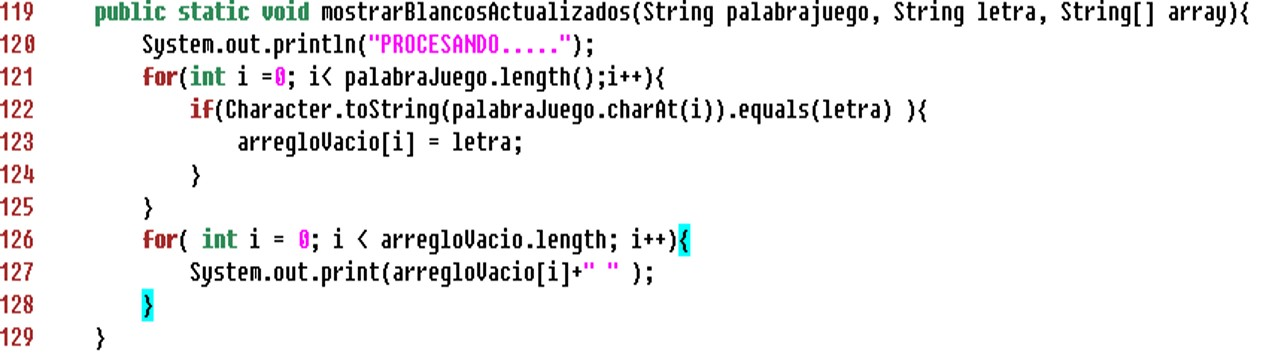
\includegraphics[width=0.8\textwidth,keepaspectratio]{img/mostrandoBlancosActualizados.jpg}
		%\includesvg{img/automata.svg}
		%\label{img:mot2}
		%\caption{Product backlog.}
	\end{figure}
	
	
	\begin{lstlisting}[language=bash,caption={Commit: Aumentando parámetros y completando el método de mostrarBlancosActualizados }]	
		git add Ejercicio02.java
		git commit -m "Aumentando parametros y completando el metodo de mostrarBlancosActualizados"
		git push -u origin main
	\end{lstlisting}
	

	
	\begin{lstlisting}[language=bash,caption={Aumentando líneas del main y determinando si se ganó o no}][H]
		vim Ejercicio02.java
	\end{lstlisting}
	
	\begin{itemize}	
		\item En la línea 74 se recibe un arreglo generado por un método. Este arreglo contiene estos elementos 
		\item En el ciclo while, se va actualizando la imagen de acuerdo a lo que el usuario ingrese. En caso el usuario logre adivinar todas las letras en los turnos previstos, el ciclo se acabará y otra forma en la que se sale ciclo es cuando se cumplen con los turnos ya establecidos
	\end{itemize}
	
	\begin{figure}[H]
		\centering
		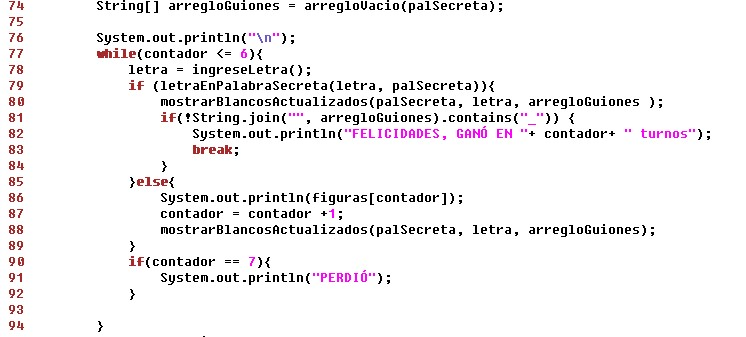
\includegraphics[width=0.8\textwidth,keepaspectratio]{img/ganador.jpg}
		%\includesvg{img/automata.svg}
		%\label{img:mot2}
		%\caption{Product backlog.}
	\end{figure}
	
	\begin{lstlisting}[language=bash,caption={Compilando Ejercicio02.java en su versión final}][H]
		javac Ejercicio02.java
		java Ejercicio02
		+---+
		|   |
		|
		|
		|
		|
		=========
		_ _ _ _ _ _ _
		
		Ingrese letra:
		o
		+---+
		|   |
		O   |
		|
		|
		|
		=========
		PROCESANDO.....
		_  _  _  _  _  _  _
		Ingrese letra:
		c
		+---+
		|   |
		O   |
		|   |
		|
		|
		=========
		PROCESANDO.....
		_  _  _  _  _  _  _
		Ingrese letra:
		p
		PROCESANDO.....
		p _  _  _  _  _  _
		Ingrese letra:
		r
		PROCESANDO.....
		p r _  _  _  _  _
		Ingrese letra:
		u
		PROCESANDO.....
		p r u _  _  _  _
		Ingrese letra:
		e
		PROCESANDO.....
		p r u e _  _  _
		Ingrese letra:
		b
		PROCESANDO.....
		p r u e b _  _
		Ingrese letra:
		a
		PROCESANDO.....
		p r u e b a _
		Ingrese letra:
		s
		PROCESANDO.....
		p r u e b a s
		FELICIDADES, HA GANADO EN 3 turnos
	\end{lstlisting}
	
	\begin{lstlisting}[language=bash,caption={Commit: Determinando el ganador y haciendo mejoras en el código }][H]
		$ git add .
		$ git commit -m "Determinando el ganador y haciendo mejoras en el codigo"			
		$ git push -u origin main
	\end{lstlisting}
	
	
	\subsection{Estructura de laboratorio 01}
	\begin{itemize}	
		\item El contenido que se entrega en este laboratorio es el siguiente:
	\end{itemize}
	
	\begin{lstlisting}[style=ascii-tree]
		lab02/
		|--- Ejercicio02.java
		|--- latex
		|----- img
		|   	|--- logo_abet.png
		|   	|--- logo_episunsa.png
		|   	|--- logo_unsa.jpg
		|   	|--- arregloSubguiones.jpg    
		|   	|--- ganador.jpg
		|		|--- letraEnPalabraSecreta.jpg
		|		|--- metodoIngreseLetra.jpg
		|----- src
		|--- programacion_lab02_rescobedoq_v1.0.pdf    
		|--- programacion_lab02_rescobedoq_v1.0.tex
		
		
	\end{lstlisting}    
	
	\section{\textcolor{red}{Rúbricas}}
	
	\subsection{\textcolor{red}{Entregable Informe}}
	\begin{table}[H]
		\caption{Tipo de Informe}
		\setlength{\tabcolsep}{0.5em} % for the horizontal padding
		{\renewcommand{\arraystretch}{1.5}% for the vertical padding
			\begin{tabular}{|p{3cm}|p{12cm}|}
				\hline
				\multicolumn{2}{|c|}{\textbf{\textcolor{red}{Informe}}}  \\
				\hline 
				\textbf{\textcolor{red}{Latex}} & \textcolor{blue}{El informe está en formato PDF desde Latex,  con un formato limpio (buena presentación) y facil de leer.}   \\ 
				\hline 
				
				
			\end{tabular}
		}
	\end{table}
	
	\clearpage
	
	\subsection{\textcolor{red}{Rúbrica para el contenido del Informe y demostración}}
	\begin{itemize}			
		\item El alumno debe marcar o dejar en blanco en celdas de la columna \textbf{Checklist} si cumplio con el ítem correspondiente.
		\item Si un alumno supera la fecha de entrega,  su calificación será sobre la nota mínima aprobada, siempre y cuando cumpla con todos lo items.
		\item El alumno debe autocalificarse en la columna \textbf{Estudiante} de acuerdo a la siguiente tabla:
		
		\begin{table}[ht]
			\caption{Niveles de desempeño}
			\begin{center}
				\begin{tabular}{ccccc}
					\hline
					& \multicolumn{4}{c}{Nivel}\\
					\cline{1-5}
					\textbf{Puntos} & Insatisfactorio 25\%& En Proceso 50\% & Satisfactorio 75\% & Sobresaliente 100\%\\
					\textbf{2.0}&0.5&1.0&1.5&2.0\\
					\textbf{4.0}&1.0&2.0&3.0&4.0\\
					\hline
				\end{tabular}
			\end{center}
		\end{table}	
		
	\end{itemize}
	
	\begin{table}[H]
		\caption{Rúbrica para contenido del Informe y demostración}
		\setlength{\tabcolsep}{0.5em} % for the horizontal padding
		{\renewcommand{\arraystretch}{1.5}% for the vertical padding
			%\begin{center}
			\begin{tabular}{|p{2.7cm}|p{7cm}|x{1.3cm}|p{1.2cm}|p{1.5cm}|p{1.1cm}|}
				\hline
				\multicolumn{2}{|c|}{Contenido y demostración} & Puntos & Checklist & Estudiante & Profesor\\
				\hline
				\textbf{1. GitHub} & Hay enlace URL activo del directorio para el  laboratorio hacia su repositorio GitHub con código fuente terminado y fácil de revisar. &2 &X &2 & \\ 
				\hline
				\textbf{2. Commits} &  Hay capturas de pantalla de los commits más importantes con sus explicaciones detalladas. (El profesor puede preguntar para refrendar calificación). &4 &X &2 & \\ 
				\hline 
				\textbf{3. Código fuente} &  Hay porciones de código fuente importantes con numeración y explicaciones detalladas de sus funciones. &2 &X &2 & \\ 
				\hline 
				\textbf{4. Ejecución} & Se incluyen ejecuciones/pruebas del código fuente  explicadas gradualmente. &2 &X &1 & \\ 
				\hline			
				\textbf{5. Pregunta} & Se responde con completitud a la pregunta formulada en la tarea.  (El profesor puede preguntar para refrendar calificación).  &2 &X &2 & \\ 
				\hline	
				\textbf{6. Fechas} & Las fechas de modificación del código fuente estan dentro de los plazos de fecha de entrega establecidos. &2 &X &2 & \\ 
				\hline 
				\textbf{7. Ortografía} & El documento no muestra errores ortográficos. &2 &X &2 & \\ 
				\hline 
				\textbf{8. Madurez} & El Informe muestra de manera general una evolución de la madurez del código fuente,  explicaciones puntuales pero precisas y un acabado impecable.   (El profesor puede preguntar para refrendar calificación).  &4 &X &2 & \\ 
				\hline
				\multicolumn{2}{|c|}{\textbf{Total}} &20 & &15 & \\ 
				\hline
			\end{tabular}
			%\end{center}
			%\label{tab:multicol}
		}
	\end{table}
	
	\clearpage
	
	\section{Referencias}
	\begin{itemize}			
		\item \url{https://drive.google.com/file/d/1MdWf_3UA_38xs18HmjPk6eH0RzRMJxkX/view?usp=drive_link}
		\item \url{https://drive.google.com/file/d/17xNjwcFykmT8BB5VbZrYEDWUg3UjLlRs/view?usp=drive_link}
	\end{itemize}	
	
	%\clearpage
	%\bibliographystyle{apalike}
	%\bibliographystyle{IEEEtranN}
	%\bibliography{bibliography}
	
\end{document}